\chapter{Odometría y SLAM}
\label{capitulo2}
\lhead{Capítulo 2. \emph{Odometría y SLAM}}

En este capítulo se presenta una revisión teórica del estado actual de las investigaciones que se han realizado en el área de odometría visual, SLAM visual, y sus vertientes en las que se fusionan los datos inerciales.

\section{Odometría}

En los últimos años se han presentado diferentes alternativas para estimar de forma efectiva el movimiento que efectúa un robot dentro de un entorno desconocido, lo cual se conoce como odometría.

En general, la odometría se encarga de estimar el movimiento de un agente (vehículo, humano, robot) utilizando sensores que pueden medir los cambios del movimiento del mismo, tales como unidades de medición inercial, láseres, cámaras, etc. El caso más simple de odometría es obtener la trayectoria recorrida por un robot diferencial a través de la lectura de los codificadores (\textit{encoders}) del robot. Los \textit{encoders} miden el desplazamiento de cada rueda, con lo que es posible obtener la orientación y el desplazamiento del robot considerando el movimiento en un plano.

Cuando se utiliza un sensor láser, la odometría se obtiene estimando el movimiento del robot mediante el escaneo y seguimiento de las medidas realizadas por el sensor (figura \ref{imagen:Antecedentes/mapa2D}).

Cuando el sensor utilizado es una cámara se denomina odometría visual (VO, del inglés: \textit{Visual Odometry}) y en este caso se puede tener la configuración monocular, en la cual se utiliza una única cámara, y la configuración estéreo, en la que se emplean dos cámaras para la estimación de movimiento. VO tiene ventajas respecto a la odometría estimada mediante \textit{encoders}, ya que no es afectada por deslizamientos de la rueda sobre la superficie en la que se desplaza el robot, y en general provee trayectorias mas precisas con errores relativos de posición de 0.1 a 2 \%. Esto hace a la odometría visual un complemento incluso a otros sistemas de navegación como el sistema de posicionamiento global (GPS), y odometría láser.

\begin{figure}[H]
	\centering
	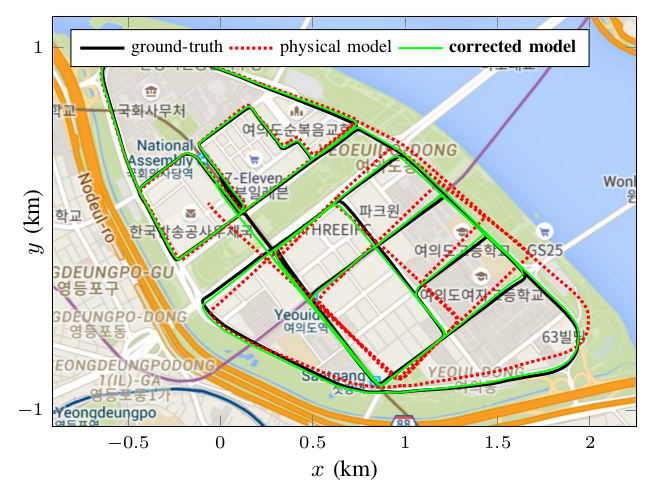
\includegraphics[scale=0.4]{EstadoDelArte/Odo/ResultadosOdo.png}
	\caption[Trayectorías estimadas por métodos de fusión de datos de \textit{encoders} y una unidad de medición inercial en un vehículo móvil en \cite{odo}]{Trayectorías estimadas por métodos de fusión de datos de \textit{encoders} y una unidad de medición inercial en un vehículo móvil en \cite{odo}. La trayectoría \textit{physical model} es la obtenida directamente por los \textit{encoders} del vehiculo. La trayectoria \textit{corrected model} es la que se obtiene a través de la fusión de los datos.}
	\label{fig:OdoEstimacion}
\end{figure}

En el caso de sensores inerciales, la orientación del robot puede obtenerse mediante la fusión de los datos del giroscopio y el acelerómetro y generalmente es utilizada en complemento con otro sensor para obtener los cambios de desplazamiento. También se utiliza fusión de los datos inerciales en conjunto con otro sensor como cámaras o \textit{encoders}. Este último caso se presenta en la figura \ref{fig:OdoEstimacion} donde la trayectoria recorrida por un vehículo es estimado mediante la integración de los datos de desplazamiento de las ruedas del vehículo en conjunto con los cambios de orientación obtenidos con la IMU.

\section{SLAM}

El problema de localización y mapeado simultáneo plantea la estimación del movimiento de un cuerpo y la construcción de un mapa de su entorno. El SLAM comparte un objetivo en común con la odometría el cual comprende estimar la trayectoria del robot. Sin embargo, la estimación  del movimiento del robot se hace en conjunto con la construcción del mapa, ya que ambos se encuentran estrechamente relacionados.

El proceso de creación del mapa consiste en adquirir la información por medio de los sensores del robot y procesarla correctamente para crear una representación 3D o 2D de su entorno. Por su parte, la localización se refiere a la estimación de la posición del robot relativo a un marco de referencia determinado. SLAM comprende a los sistemas que efectúan ambos procesos de forma simultánea.

Esta relación entre mapa  y localización del robot  fue inicialmente establecida en un artículo presentado en el \textit{International Symposium on Robotics Research} \cite{HarrisAndStephens} cuando se estableció que integrar la estimación de la localización y el mapeado del entorno de forma simultánea en un mismo problema, tenía un resultado convergente, cuya convergencia además aumentaba al existir un número mayor de puntos de referencia. 


Durante el periodo 1986-2004, se introdujeron métodos de estimación probabilistas  como los filtros extendidos de Kalman (EKF, del inglés: \textit{Extended Kalman Filter}), filtros de partículas Rao-Blackwell y estimaciones de máxima verosimilitud. Además surgieron vertientes de SLAM ligadas a la inteligencia artificial, toma de decisiones de robots y teoría de control, la cual es conocida como SLAM activo. Algunos trabajos resaltantes son \cite{Feder, Smith, Makarenko, Stachniss}.

El SLAM moderno se compone de dos módulos principales: el módulo de sensores (front end) y el módulo de optimización (back end). El front end se encarga de extraer la información de los sensores y realizar las estimaciones a \textit{priori} del movimiento. El modulo de back-end se encarga de refinar las estimaciones utilizando optimización no lineal para generar una solución mas robusta y consistente entre el mapa y el recorrido. Este último módulo comprende la estimación \textit{posteriori} (MAP, del inglés: \textit{Maximum a Posteriori}). Estos módulos se ilustran en la figura \ref{fig:SLAMStruct}.

\begin{figure}[H]
	\centering
	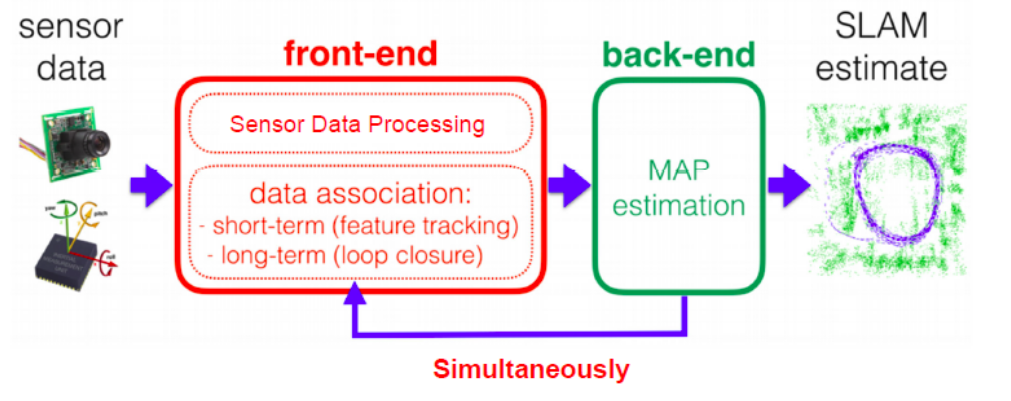
\includegraphics[scale=0.4]{EstadoDelArte/SLAM/FrontEndAndBackEnd.png}
	\caption[Estructura general del SLAM]{Estructura general del SLAM. El \textit{front-end} representa el modulo de procesamiento de datos generando las estimaciones \textit{a priori} del movimiento. El modulo de back-end se encarga de realizar la optimización global del recorrido y del mapa \cite{Cadena}}.
	\label{fig:SLAMStruct}
\end{figure}

%A lo largo de los años se ha mejorado la eficiencia y robustez en la optimización del problema, por ejemplo con métodos de suavizaje por factorización [20, 44],
%filtrado para marginalizar estimaciones y resumir la información pasada [74], y op-
%timización de redes de mapas y posiciones estimadas [37, 80]. Todos estos enfoques
%utilizan MAP como método de estimación, y a menudo usan un grafo de factores
%(factor graph) para representar la información conocida del problema, con nodos
%que corresponden a las variables (las posiciones del robot y las posiciones de los
%puntos de referencia) y factores que definen las dependencias existentes entre dis-
%tintos nodos. La interpretación como un grafo de factores tiene como ventaja darle
%organización, generalidad y perspectiva al problema de SLAM, además de permitir
%la fácil inclusión de las restricciones existentes al problema de optimización.


Como se muestra en la figura \ref{fig:SLAMGraph}, el problema de SLAM se puede considerar como un grafo de factores. Los círculos azules representan posiciones estimadas del robot en tiempos consecutivos, mientras que los círculos verdes representan las posiciones de los puntos de referencia. Los círculos rojos representan las variables secundarias asociadas a la percepción de los puntos de referencia. Los factores están mostrados como cuadrados negros: donde  “u” representan las restricciones correspondientes a odometría, “v” factores correspondientes a las observaciones, “c” cierres de lazo, y “p” factores pasados.


%GTSAM [21], g2o [48], Ceres [2], iSAM [44] y SLAM++ [68]


\begin{figure}[H]
	\centering
	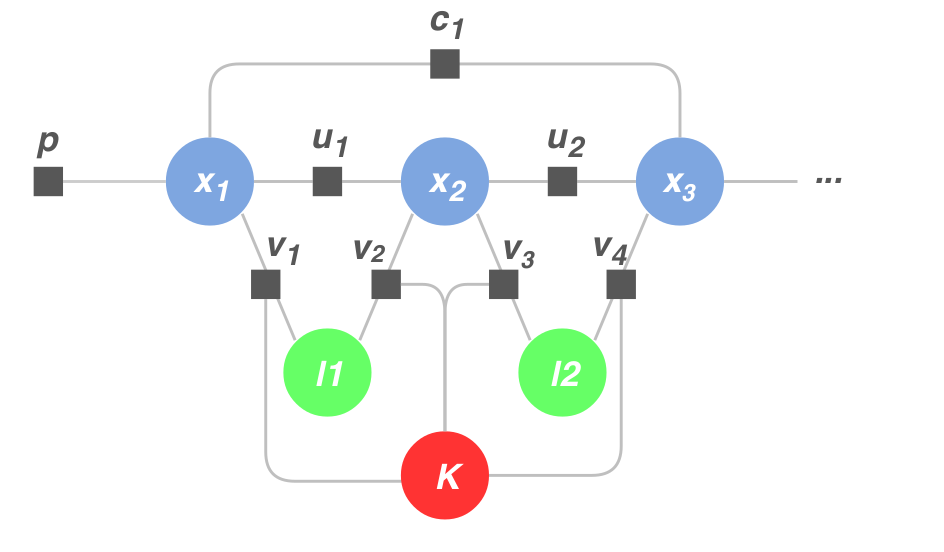
\includegraphics[scale=0.4]{EstadoDelArte/SLAM/Graph.png}
	\caption{Problema de SLAM representado como un grafo de factores \cite{Cadena}}.
    \label{fig:SLAMGraph}
\end{figure}



\section{Odometría  y SLAM visual}

Los métodos de odometría y SLAM visual, se dividen en los métodos directos e indirectos. A continuación se presentan algunos trabajos en el área.

\subsection{Métodos indirectos}

Los métodos indirectos son aquellos que se basan en detectar puntos de interés en las imágenes, y en estimar el movimiento del robot en función de las parejas de correspondencias entre imágenes de dichos puntos de interés.

En general, estos métodos utilizan detectores y extractores de puntos de interés (FAST, ORB, SIFT, SURF, KAZE ó AKAZE), los cuales se encargan de clasificar una región de la imagen como punto de interés, y de dar la ubicación en píxeles del punto característico. Posteriormente se utilizan emparejadores, los cuales comparan los puntos de interés entre imágenes y generan las mejores parejas entre los conjuntos. Las parejas correctas poseen puntos característicos de diferentes imágenes, que representan a la misma región u objeto dentro de las imágenes (por ejemplo, esquinas similares). 

La estimación de movimiento se realiza en función de estas parejas, utilizando el modelo de la cámara. Para ello pueden ser utilizados métodos de optimización que minimizan del error de reproyección entre parejas, o métodos como RANSAC, que permite hallar la transformación de movimiento que reduce el error de un subconjunto de las parejas y ademas permite el filtrado de las correspondencias erróneas.

Los métodos de SLAM visual indirectos hacen un seguimiento de las correspondencias a través de múltiples imágenes para realizar una construcción del mapa del entorno del robot. En general se utilizan grafos para estimar la mejor relación entre mapa y movimiento del robot a medida que se introducen nuevas observaciones. Un sistema de localización y mapeo simultáneo destacado se presenta a continuación:


\subsubsection{ORB-SLAM}

En el año 2015 Tardos et al. \cite{orbSlam}, pertenecientes al Instituto de Investigación de Ingeniería de Aragón, en la Universidad de Zaragoza,  desarrollaron ORB-SLAM, el cual es el sistema de código abierto de SLAM visual más robusto basado en métodos indirectos. Su nombre se debe a la utilización del detector ORB para garantizar la ejecución en tiempo real.

ORB-SLAM utiliza tres hilos en CPU para resolver de forma simultánea la estimación de movimiento, el mapeado local y el cierre de lazo.

En los sistemas monoculares, un problema común es la estimación del mapa inicial, el cual se basa en escoger un par de imágenes con suficiente disparidad entre ellas, para triangular sus correspondencias. En algunos sistemas esta selección inicial de imágenes se realiza de forma manual. En el caso de ORB-SLAM, se utiliza un algoritmo de inicialización automática del mapa, el cual es capaz de discernir movimientos en escenas planas y no planas mediantes el cálculo de la matríz esencial y de homografia. Cuando se detecta movimiento sobre una escena plana, la estimación de movimiento entre las dos imágenes se realiza utilizando la matríz de homografía. Cuando el movimiento es sobre una escena con objetos de diferentes profundidades, la estimación se realiza mediante el empleo de la matriz esencial.  De esta forma, con el movimiento estimado entre el par de imágenes, es posible obtener el mapa inicial sin necesidad de intervención humana.

Posteriormente se elaboró ORB-SLAM2 \cite{orbSlam2}, el cual permite la implementación de cámaras estereoscópicas y cámaras RGB-D,
lo cual permitió aumentar de forma considerable la información disponible del entorno, aumentando la densidad de los mapas generados y mejorando la precisión de las estimaciones del mapa y del movimiento del robot.


\subsection{Métodos directos}

Los métodos directos visuales utilizan la intensidad de luz capturada en la imagen de la cámara como para estimar el movimiento del robot basado en algún método que utilice como función de error la diferencia fotométrica entre imágenes. 

Los métodos directos pueden utilizar toda la información disponible al utilizar toda la región de la imagen, o parte de ella al procesar sólo parches de la imagen. Las reconstrucciones generadas pueden ser densas, en los casos en que se utiliza la mayor cantidad de información posible, y semidensas cuando se utilizan parches. En las reconstrucciones densas los mapas generados presentan una reconstrucción bastante completa del entorno y de sus objetos, y en los mapas semidensos se genera una reconstruccion parcial.

Por supuesto que el costo computacional es mayor al analizar mayor cantidad de regiones en la imagen, por lo que en general los metodos de SLAM utilizan reconstrucciones semidensas, mientras que los métodos de reconstrucción offline utilizan reconstrucción densa.

Entre los métodos indirectos de SLAM visual más representativos en los últimos
años están: 

\subsubsection{DSO}

En el año 2017 fue desarrollado DSO (\textit{Direct Sparse Odometry}) \cite{DSO}, la cual es una implementación enfocada en reconstrucciones dispersas en tiempo real usando CPU,  lo cual permite ser empleado en dispositivos como computadoras portátiles. 
	
DSO utiliza métodos directos que utilizan el error fotométrico definido directamente en las imágenes y optimización no lineal. El sistema de optimización engloba las variables asociadas a la posición de la cámara, parámetros intrínsecos, y parámetros geométricos (estimaciones de profundidad de los puntos).La optimización se realiza de manera local en una ventana que engloba únicamente a un grupo reciente de imágenes clave, y marginaliza posiciones muy antiguas de la cámara y los puntos que ya no están dentro del campo de visión actual de la cámara. 


\begin{figure}[H]
	\centering
	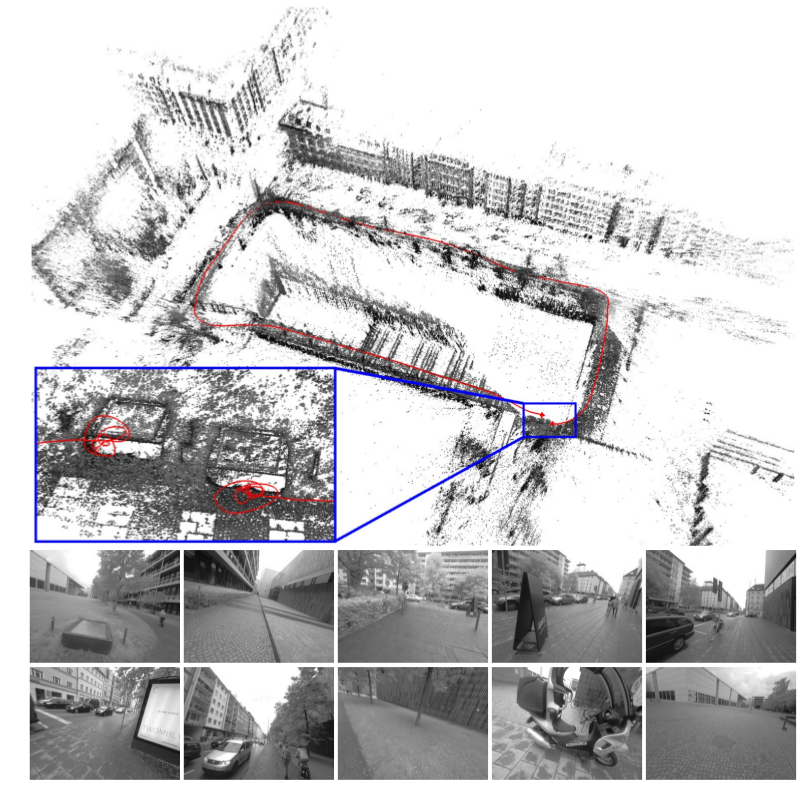
\includegraphics[scale=0.4]{EstadoDelArte/DSO/dso.png}
	\caption[Resultados obtenidos utilizando DSO \cite{DSO}] {Resultados obtenidos utlizando DSO \cite{DSO}. En la parte superior se presenta el mapa reconstruido alrededor de un edificio utilizando un video de 100 segundos utilizando cámara monocular . El cuadro azul representa la vista de cerca del punto de inicio y final del recorrido, donde se observa el error acumulado en el curso de la trayectoria. En la parte inferior se presentan una selección de imágenes del video en cuestión.}
	\label{fig:DSOEstimacion}
\end{figure}

DSO emplea la parametrización de la posición de la cámara mediante el grupo
de álgebra de Lie, y toma en cuenta las características fotométricas de la cámara, como la atenuación de los lentes, la corrección del gamma y la velocidad de obturación. Esto permite aumentar la precisión y robustez de los resultados.


Las imágenes procesadas en DSO se dividen en cuadrículas, donde puntos con
alta intensidad de gradiente, superiores a un límite adaptable, son seleccionados
como candidatos para su seguimiento y la estimación de la profundidad. Este
método de cuadrícula  permite obtener una distribución uniforme de puntos en
toda la imagen, mejorando el mapa y la trayectoria estimada. El límite que define
si un punto es considerado de alta intensidad o no, está determinado por el número
de puntos encontrados en cada cuadrícula, y es modificado para obtener un número
de puntos relativamente constante durante todo el proceso.

	
En comparación con ORB-SLAM, este último ofrece un sistema más completo y general, ya que DSO está diseñado para odometría visual, y no ofrece una optimización global del mapa. Sin embargo, si se limitan las características de optimización global y relocalización de ORB-SLAM,  DSO obtiene resultados cercanos en robustez y
precisión a los de ORB-SLAM. En general, ORB-SLAM presenta mejores resultados cuando las secuencias de datos contienen casos en los que la cámara regresa al mismo lugar donde estaba, lo que permite a ORB-SLAM realizar cierres de lazo que eliminan la deriva (\textit{drift}) acumulada.


%Newcombe et al. propusieron un método completamente directo de SLAM vi-
%sual llamado DTAM [60]. DTAM utiliza la información de todos los pı́xeles de la
%imagen (enfoque completamente denso) para generar reconstrucciones continuas
%del entorno. La alta demanda computacional que esto exige hace posible la ejecu-
%ción en tiempo real de DTAM si se emplea una unidad de procesamiento gráfico
%(GPU, del inglés: Graphics Processing Unit).
%La estimación de la posición de la cámara (con seis grados de libertad) es
%obtenida a partir de la alineación densa de imágenes sintéticas generadas a partir
%del mapa reconstruido, minimizando el error fotométrico entre ellas. De forma
%paralela, a partir de imágenes nuevas se realiza un proceso de actualización yCapı́tulo 2. Revisión del estado del arte
%23
%expansión del modelo denso del mapa, que permite alcanzar precisión de sub-
%pı́xeles en las reconstrucciones obtenidas.
%Figura 2.7: Reconstrucciones de los mapas de profundidad densos utilizando
%DTAM [60].
%DTAM optimiza el mapa reconstruido asumiendo continuidad en el espacio,
%por lo que las coordenadas en tres dimensiones de todos los pı́xeles pueden ser
%calculadas. La inicialización del mapa se realiza usando mediciones entre pares de
%imágenes, al igual que PTAM, usando el algoritmo de cinco-puntos. Al obtener
%la primera imagen clave del sistema, la reconstrucción cambia al enfoque denso
%explicado. En la Figura 2.7 se observan resultados de DTAM utilizando una GPU
%NVIDIA GTX 480, un procesador i7 quad-core CPU y una cámara RGB con
%resolución de 640 x 480.

\section{Fusión visual-inercial }
A lo largo de los años se han utilizado diferentes tipos de sensores y sus combinaciones para realizar la localización y mapeo simultáneo (SLAM) de un robot móvil en su entorno. Entre éstos se encuentran láseres de rango, sonares, sistemas de posicionamiento global (GPS), unidades de medición inercial (IMU) y cámaras monoculares, estereoscópicas, y RGB-D.

Cada tipología en la que son empleados estos sensores tiene sus limitaciones. Por ejemplo, los sistemas en que los se utiliza GPS están restringidos a ser utilizados al aire libre, lo que conlleva a que no puedan ser empleados en vehículos submarinos. Los láseres ofrecen información precisa del entorno pero tienen problemas en superficies reflectivas o absorbentes, además que pueden representar un alto costo,  y  ser lo suficientemente pesados como para ser descartados en aplicaciones con  vehículos aéreos. Por su parte, las medidas de sonares que son aplicados en espacios terrestres pueden tener alta incertidumbre ya que depende de la forma de las superficies y de su orientación relativa al sensor, mientras que las unidades de medición inercial presentan deriva y ruido en sus mediciones. En el caso de las cámaras, la  calidad de sus datos tienen una alta dependencia a las condiciones de iluminación. 

La implementación de estas últimas en sistemas de localización y mapeo simultáneo ha tenido gran atención en los últimos años debido a su capacidad para capturar una gran cantidad de información sobre el entorno. Es por esto que se han desarrollado métodos de SLAM visual basados tanto en cámaras monoculares como estereoscópicas, utilizando para ello métodos directos, a través de la detección y emparejamiento de características en las imágenes; método indirectos, basados en el calculo del error fotométrico entre imágenes; y semi-directos, utilizando una combinación de métodos directos e indirectos.

Sin embargo, estos sistemas presentan debilidades. Los métodos de SLAM con cámaras monoculares presentan problemas de ambiguedad ante la escala, mientras que  los estereoscópicos están limitados por la relación entre la profundidad de la escena y la distancia entre las cámaras. 

Es por ello que con el objetivo de generar un sistema más robusto en el que se puede complementar la información disponible entre sensores y compensar sus debilidades, se han propuesto esquemas basados en la fusión visual-inercial, en la que se pueden emplear cámaras estéreos o monoculares junto a una unidad de medición inercial, ofreciendo además una buena relación entre costo, peso, espacio ocupado y consumo de energía, que permite que puedan ser empleados en robots terrestres, aéreos y submarinos.

El núcleo de esta fusión se encuentra basado en la complementariedad que tienen estos sensores. Por ejemplo, las cámaras son precisas en movimientos lentos, en los cuales las medidas aceleración y velocidad angular provenientes de la IMU tienen mayor incertidumbre. En el caso de movimientos rápidos, sucede justo lo contrario: la IMU presenta menor incertidumbre en sus medidas mientras que las imágenes captadas por la cámara se distorsionan por efectos como el blur. 

Por otro lado,  las frecuencias de muestreo de las cámaras convencionales están el orden de las decenas de Hertz, mientras que las de la IMU pueden alcanzar las centenas de Hertz, con lo que se  obtiene información inercial adicional entre dos imágenes, que al ser integrada permite establecer restricciones de movimiento,  logrando de esta forma alcanzar una mejor estimación del estado del robot frente a su entorno., requiriendo un menor tiempo de cómputo. 



\section{SLAM visual inercial}

Los sistemas de SLAM y de odometría tienden a ser más robustos a medida que se añaden más sensores al sistema. Este es el caso del SLAM visual inercial, donde se utiliza visión estéreo o monocular en conjunto con una unidad de medición inercial, para estimar el movimiento del robot y el mapa de su entorno.  La complementariedad de los sensores permite que puedan ser implementados metodos visuales directos en conjunto con las mediciones de la IMU, las cuales se relacionan directamente con la orientación del robot y los cambios de rotación. Además, al utilizar las medidas de aceleración de la IMU es posible obtener el factor de escala absoluta  del mapa estimado y de la trayectoria del robot, la cual no es posible de obtener en los sistemas meramente monoculares. Esto fue demostrado a través a través de un filtro EKF que permite la fusión de los datos inerciales y visuales en el artículo de  Scaramuzza et al. \cite{scaramuzza}.

A continuación se presentan los trabajos más destacados en Odometría y SLAM visual inercial.

\subsection{OKVIS}

El sistema de SLAM visual-inercial basado en keyframes y optimización no lineal (OKVIS)  es un enfoque desarrollado en 2013 en el laboratorio d de sistemas autónomos de la Escuela Politécnica Federal de Zúrich (ETH), en Suiza, por  Leutenegger S. et al \cite{okvis}.


Este enfoque integra de forma estrecha las medidas de la IMU y los keyframes provenientes de visión estéreo, utilizando optimización de Gauss-Newton donde los estados del sistema incluyen la posición, velocidad y orientación del robot, así como también los sesgos de la IMU. El detector que se empleó es el detector de Harriz multiescala con optimización en el espacio SSE , combinado con el descriptor BRISK. 

La visión estereo es utilizada para realizar la triangulación de los puntos característicos en cada frame, los cuales son insertados a un mapa local. Luego se aplica el algoritmo de fuerza bruta para encontrar la correspondecia con el mapa global de landmarks. En este caso, se utiliza outlier rejection aplicnado es test de chi-cuadrado a las coordenadas de la imagen utilizando las poses obtenidas previamente mediante la integración de las medidas de la IMU.
En este enfoque se utiliza una ventana deslizante para mantener las imágenes (\textit{frames}) más recientes, y la selección de imágenes claves (\textit{keyframes}) se basa en una medida heurística: si la razón entre el área ocupado por todo los puntos emparejados contra el area ocupa por todos los puntos detectados está entre 50 a 60, el frame es considerado como keyframe.

Debido a que se utiliza keyframes, se pueden tener frames separados arbitrariamente en tiempo. 

En este trabajo comparan las estimaciones realizadas entre los diferentes acoples: el visual, el ligeramente acoplado y el estrechamente acoplado. la figura \ref{fig:RovioEstimacion} y \ref{fig:RovioEstimacionMapa} presenta los resultados obtenidos.

\begin{figure}[H]
	\centering
	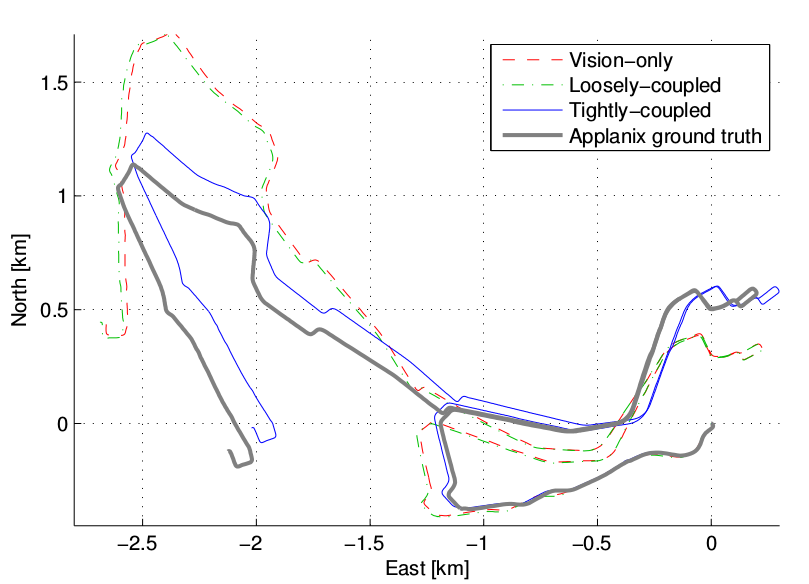
\includegraphics[scale=0.4]{EstadoDelArte/Okvis/OkvisResultados.png}
	\caption[Resultados comparativos de la estimación del recorrido de un vehículo  en \cite{okvis}]{Resultados comparativos de la estimación del recorrido de un vehículo  en \cite{okvis} . El enfoque Tighly-couple representa el método implementado en Okvis. El enfoque Loosely-Coupled representa un acople en menor grado de las medidas de IMU y cámara. Visión-only representa el enfoque basado sólo en cámara. El groundtruth es mostrado en gris.}
	\label{fig:RovioEstimacion}
\end{figure}


\begin{figure}[H]
	\centering
	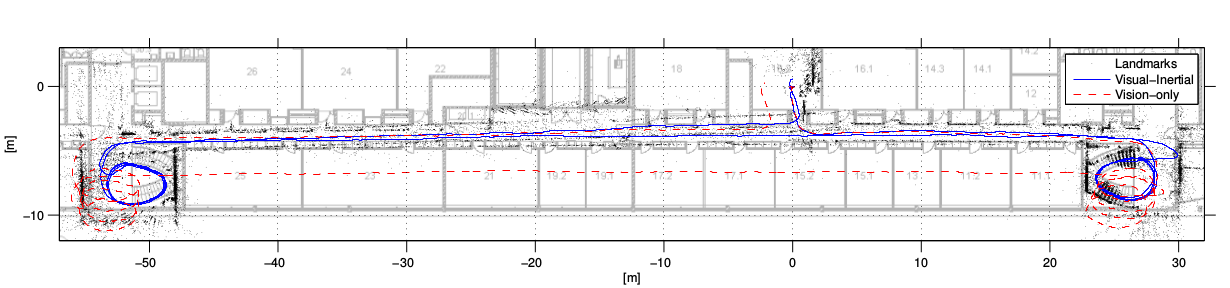
\includegraphics[scale=0.4]{EstadoDelArte/Okvis/OkvisMapa.png}
	\caption[Vista ortonormal de la reconstrucción del camino realizado en un edificio utilizando OKVIS]{Vista ortonormal de la reconstrucción del camino realizado en un edificio utilizando OKVIS. Las trayectorias se encuentran manualmente alineada con el plano de la estructura.}
	\label{fig:RovioEstimacionMapa}
\end{figure}


\subsection{ROVIO}

La Odometría Visual-Inercial Robusta (ROVIO, del inglés: \textit{Robust Visual Inertial Odometry}) es un algoritmo desarrollado en 2015 en el laboratorio de sistemas autónomos del ETH.

Este algoritmo utiliza directamente como error la intensidad de los píxeles, utilizando parches en las  imágenes y aplicando la estructura piramidal de 4 niveles y manteniendo un alto nivel de robustez. Los parches utilizados están fuertemente acoplados con un filtro Kalman Extendido (EKF, del inglés: \textit{Extended Kalman Filters}) y los landmarks 3D son siempre estimados con respecto a la pose actual de la cámara. lo que es conocido como el enfoque robocéntrico. Además, estos landmarks son parametrizados para lograr una na forma compacta de representación y de esa forma mejorar el desempeño computacional del algoritmo. 

El filtro empleado fusiona los datos de aceleración y velocidad angular de la IMU, y los parámetros extrinsecos de la cámara y los biases de la IMU son coestimados. 

Las características utilizadas aquí se refieren directamente a un píxel dentro de un parche de la imagen. El propósito del filtro es predecir la ubicación de las características en la siguiente imagen y de esta forma, extraer un parche de la siguiente imagen, y estimar la mejor transformación de cuerpo rígido que minimice el error de intesidad entre los parches. 

Cuando la predicción de la ubicación del parche se encuentra fuera de la región de la imagen, es eliminada la características y se crean nuevas. También puede ser eliminada la caracteristica en función de sus estadísticas, las cuales están asociadas al grado de certidumbre o varianza. La imagen \ref{fig:RovioEstimacion} muestra un ejemplo de esto.

\begin{figure}[H]
	\centering
	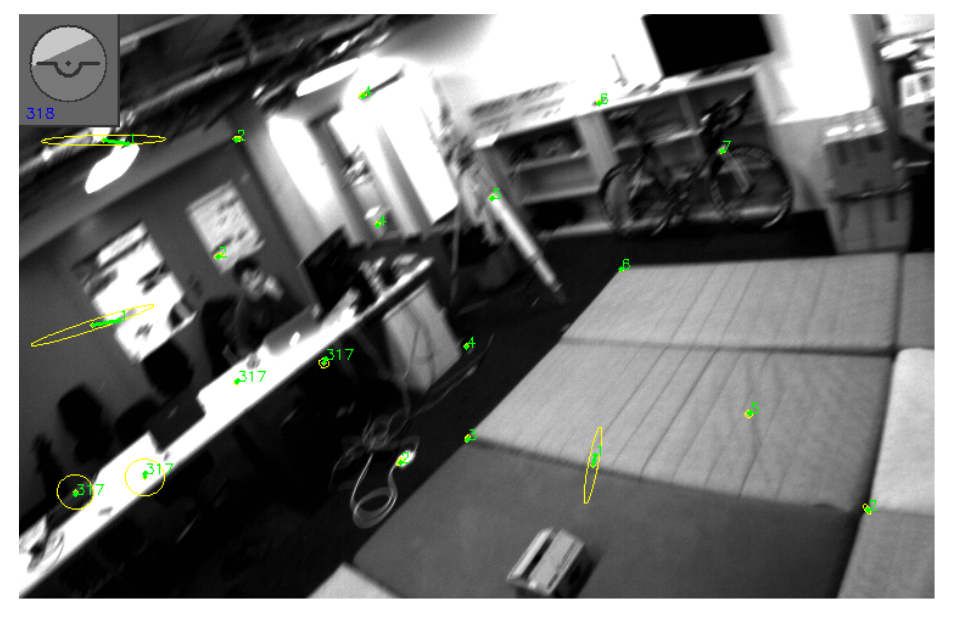
\includegraphics[scale=0.4]{EstadoDelArte/Rovio/RovioEstimacion.png}
	\caption[Captura del entorno de trabajo de la odometría visual-inercial]{Captura del entorno de trabajo de la odometría visual-inercial. Las elipses encierran la zona donde se predice la localización de las características. Las elipses estrechas corresponden a las características de mayor incertidumbre, entre las que se encuentran las características nuevas. Luego de la estimación efectuada por el EKF, la localización de la característica es mostrada como un punto verde. Los números en color verde corresponden al número de veces que ha sido seguida la características (1 si es una nueva característica).}
	\label{fig:RovioEstimacion}
\end{figure}


Este enfoque no requiere una etapa de inicialización, por lo que es posible utilizar este sistema de estimación de estados directamente. Para evaluar la robustez de este algoritmo, el laboratorio utilizo su propio vehiculo aerio, equipado con dos cámaras con disparo global sincronizadas con el trigger de la IMU. En el contexto del trabajo sólo fue utilizado una de las cámaras. El Ground truth fue proveido por un sistema externo de captura de movimiento. En esta configuración se fijó la tasa de las medidas de la IMU a 200Hz y la de las cámaras a 20Hz. Los resultados de la estimación se presentan en las figuras \ref{fig:RovioOrientacion} y  \ref{fig:RovioTrayectoria}.

\begin{figure}[H]
	\centering
	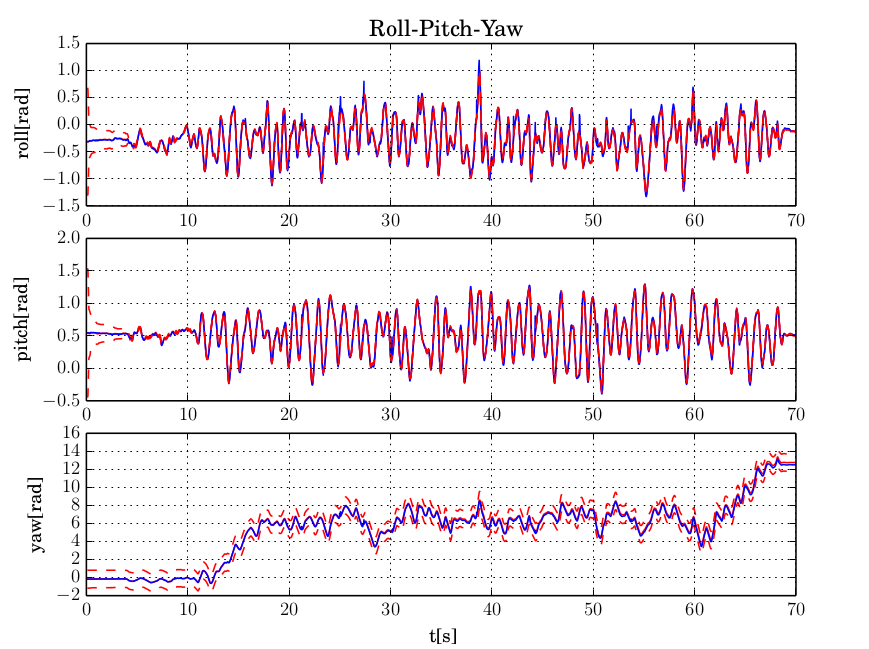
\includegraphics[scale=0.4]{EstadoDelArte/Rovio/RovioOrientacion.png}
	\caption[Ángulos RPY estimados utilizando ROVIO]{Ángulos RPY estimados (rojo) del UAV comparado con los obtenidos mediante el sistema de captura de movimiento (azul). La incertidumbre de la estimación se muestra con lineas discontinuas. }
	\label{fig:RovioOrientacion}
\end{figure}


\begin{figure}[H]
	\centering
	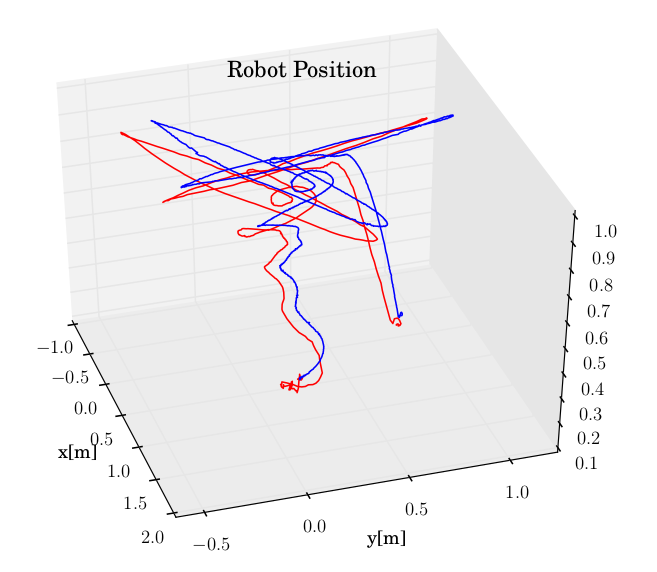
\includegraphics[scale=0.4]{EstadoDelArte/Rovio/RovioTrayectoria.png}
	\caption[Trayectoria estimada utilizando ROVIO]{Trayectoria estimada (rojo) del UAV comparado con el groundtruth (azul) proveniente del sistema de captura de movimiento .}
	\label{fig:RovioTrayectoria}
\end{figure}



\section{EuRoC MAV Dataset}

El conjunto de datos de prueba empleado en este trabajo corresponde al al EuRoC MAV Dataset \cite{euroc}, el cual es un dataset de referencia que es utilizado para evaluar diferentes algoritmos de SLAM visual-inercial y que dispone de 11 secuencias de datos. \\


El EuRoC MAV Dataset contiene imágenes estéreo sincronizadas con las medidas de la IMU,  y un groundtruth preciso que es estimado utilizando el láser Leica y el sistema de captura de movimiento Vicon. Los datos fueron recolectados utilizando robot aéreo el cual se presenta en la figura \ref{fig:robotEuroc}. \\

\begin{figure}[H]
	\centering
	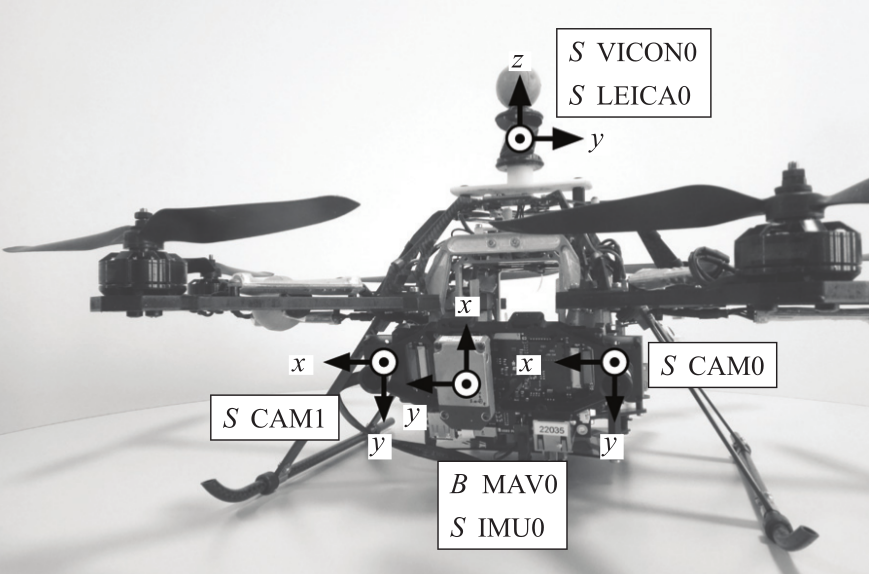
\includegraphics[scale=0.4]{Implementacion/robotEuroc.png}
	\caption[Robot aéreo empleado en la recolección de datos en el EuRoC MAV Dataset]{Robot aéreo empleado en la recolección de datos en el EuRoC MAV Dataset.}
	\label{fig:robotEuroc}
\end{figure}

Las cámaras empleadas en estas secuencias capturan datos a 20Hz, mientras que la IMU opera a 200Hz. En nuestro caso, se utilizará la cámara CAM0 de la figura \ref{fig:robotEuroc}. Esta cámara se encuentra sincronizada con la IMU tal como se presenta en la figura \ref{fig:sincronizacionEuroc}. En un tiempo $t_k$ se captura tanto la imagen de la cámara, como las medidas de aceleración y velocidad angular provenientes de la IMU. El tiempo $t_c$ representa el lapso de tiempo entre la captura de dos imágenes y corresponde con 50 ms. En este caso, se tienen $n = 10$ medidas de la IMU entre cada captura de la cámara. \\

\begin{figure}[H]
	\centering
	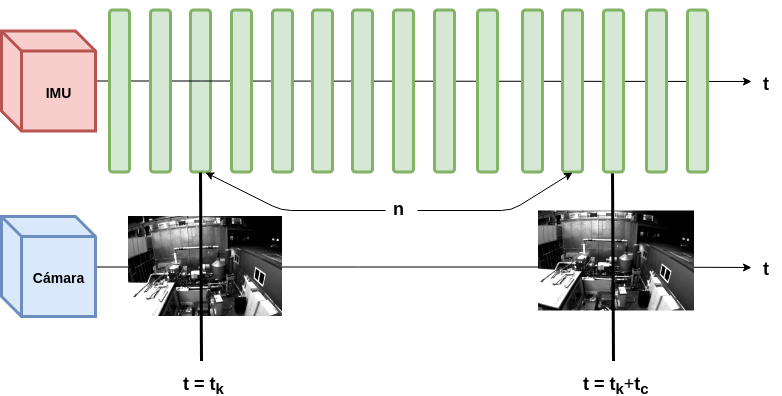
\includegraphics[scale=0.4]{Implementacion/DiagramaIMUCamara.png}
	\caption[Sincronización entre la IMU y la cámara]{Sincronización entre la IMU y la cámara.}
	\label{fig:sincronizacionEuroc}
\end{figure}

También se dispone de la calibración de los parámetros intrísecos y extrinsecos del sistema. En la figura \ref{fig:extrinsecosEuroc} se muestran los parámetros extrínsecos relevantes para este trabajo. En este caso, se utiliza la transformación de cuerpo rígido $T_{BCAM0}$, que relaciona el sistema de referencia de la IMU (Body, B) y el sistema de referencia de la cámara CAM0. 



\begin{figure}[H]
	\centering
	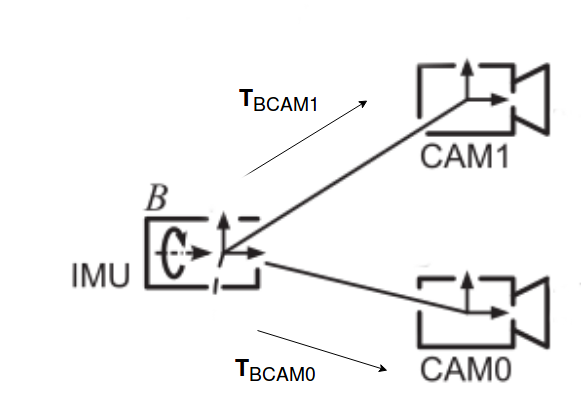
\includegraphics[scale=0.4]{Euroc/Enlaces.png}
	\caption[Parámetros extrínsecos del sistema]{Parámetros extrínsecos del sistema.}
	\label{fig:extrinsecosEuroc}
\end{figure}

Las secuencias de este conjuntos de datos se encuentran clasificadas en ``fácil'', ``media'', y ``difícil'',  en función de la media de la velocidad lineal y angular del robot utilizado y de las condiciones visuales y niveles de iluminación. En la figura \ref{fig:tablaDeCaracteristicas} se presentan las características de las secuencias. 

\begin{figure}[H]
	\centering
	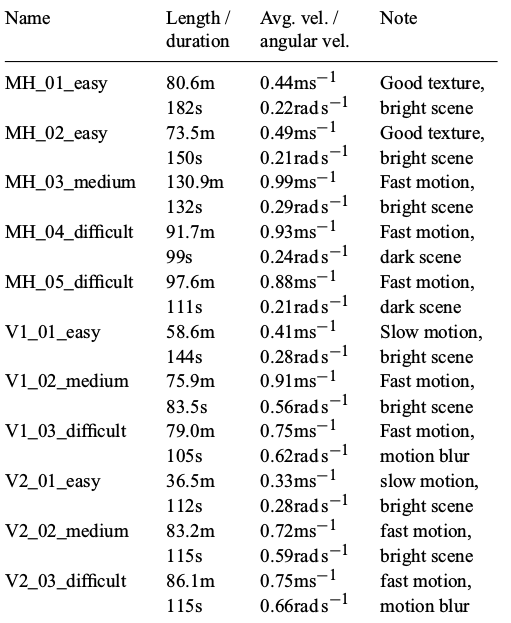
\includegraphics[scale=0.4]{Euroc/TabladeCaracteristicas.png}
	\caption[Características de las secuencias de datos del EuRoC MAV Dataset]{Características de las secuencias de datos del EuRoC MAV Dataset.}
	\label{fig:tablaDeCaracteristicas}
\end{figure}



Este conjunto de datos fue recolectado en dos tipos de ambiente. El primer ambiente se presenta en la figura \ref{fig:machineHall} y  corresponde a una sala de máquinas en el cual fueron recolectadas 5 secuencias de datos (MH\_01\_easy, MH\_02\_easy, MH\_03\_medium, MH\_04\_difficult, MH\_05\_difficult). \\

En la figura \ref{fig:vicon} se muestra el segundo ambiente correspondiente a una habitación en el que se tomaron 6 secuencias de datos (V1\_01\_easy, V1\_02\_medium, V1\_03\_difficult, V2\_02\_easy, V2\_02\_medium, V2\_03\_difficult). En estas secuencias se dispone de la nube de puntos de la habitación, la cual fue generada a través de la fusión de las medidas tomadas con el láser Leica, y se presentan en la figura \ref{fig:pointcloudEuroc}.\\

\begin{figure}[H]
	\centering
	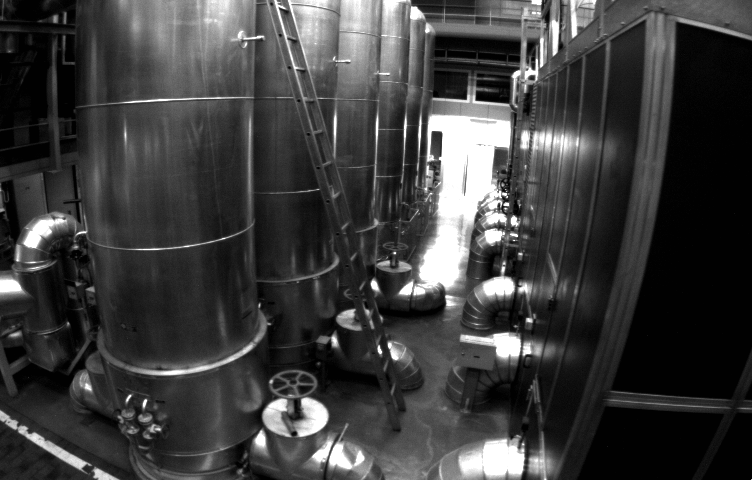
\includegraphics[scale=0.2]{Euroc/MachineHall1.png}
	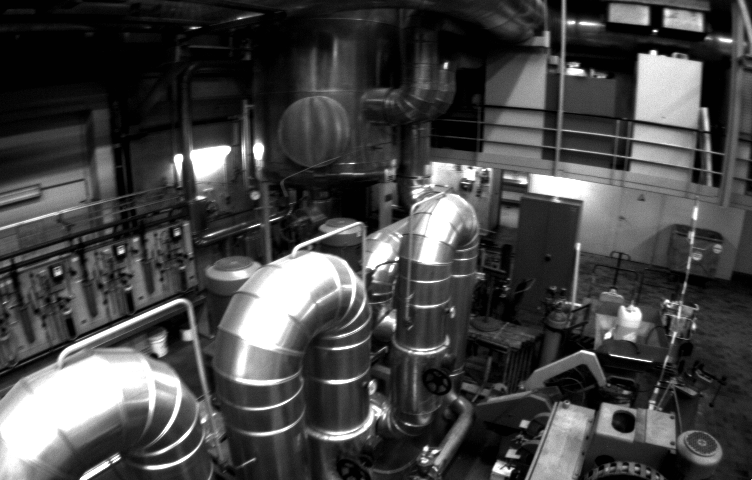
\includegraphics[scale=0.2]{Euroc/MachineHall2.png}
	\caption[Imágenes de la secuencia de datos correspondiente a la sala de máquinas]{Imágenes de la secuencia de datos correspondiente a la sala de máquinas.}
	\label{fig:machineHall}
\end{figure}


\begin{figure}[H]
	\centering
	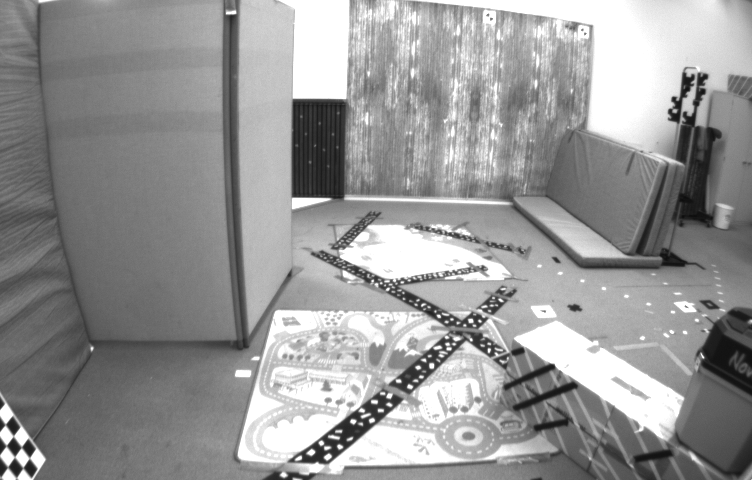
\includegraphics[scale=0.2]{Euroc/Vicon0.png}
	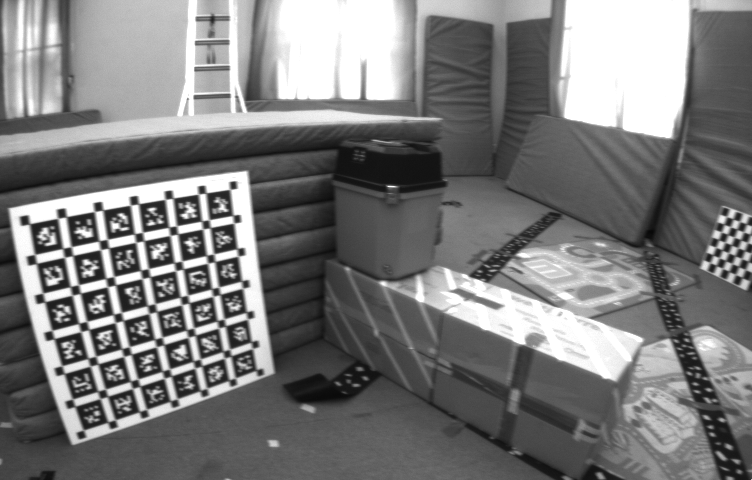
\includegraphics[scale=0.2]{Euroc/Vicon1.png}
	\caption[Imágenes de la secuencia de datos correspondiente a la habitación Vicon]{Imágenes de la secuencia de datos correspondiente a la habitación Vicon.}
	\label{fig:vicon}
\end{figure}


\begin{figure}[H]
	\centering
	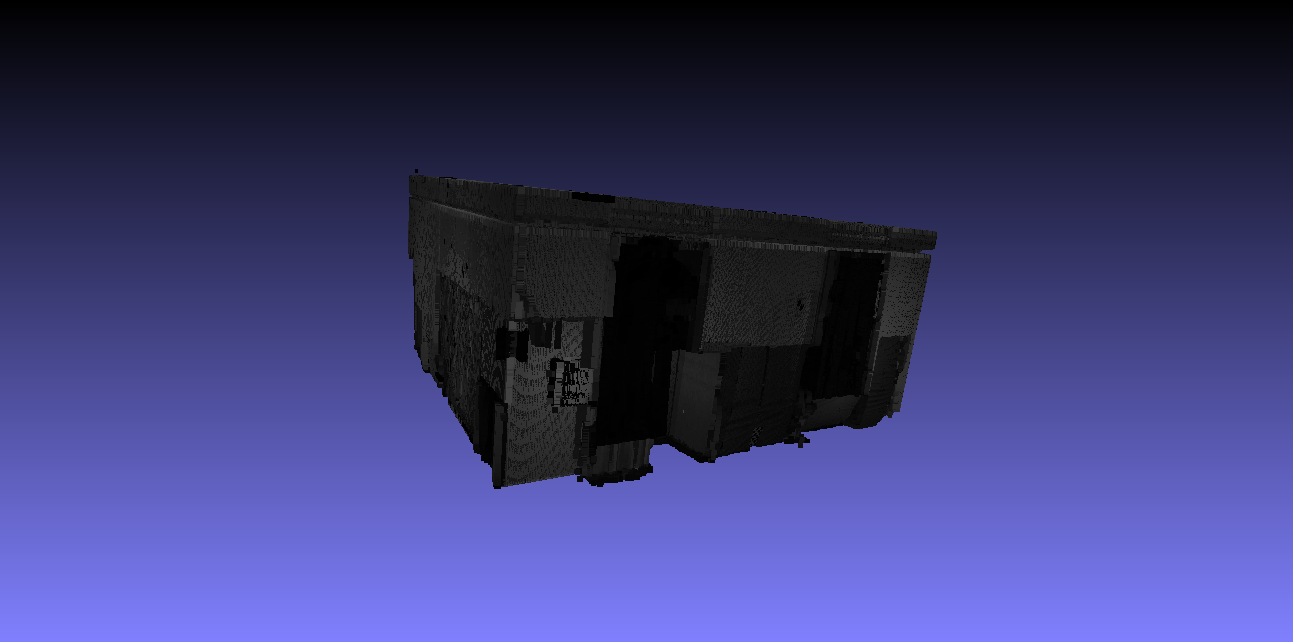
\includegraphics[scale=0.2]{Euroc/Pointcloud0.png}
	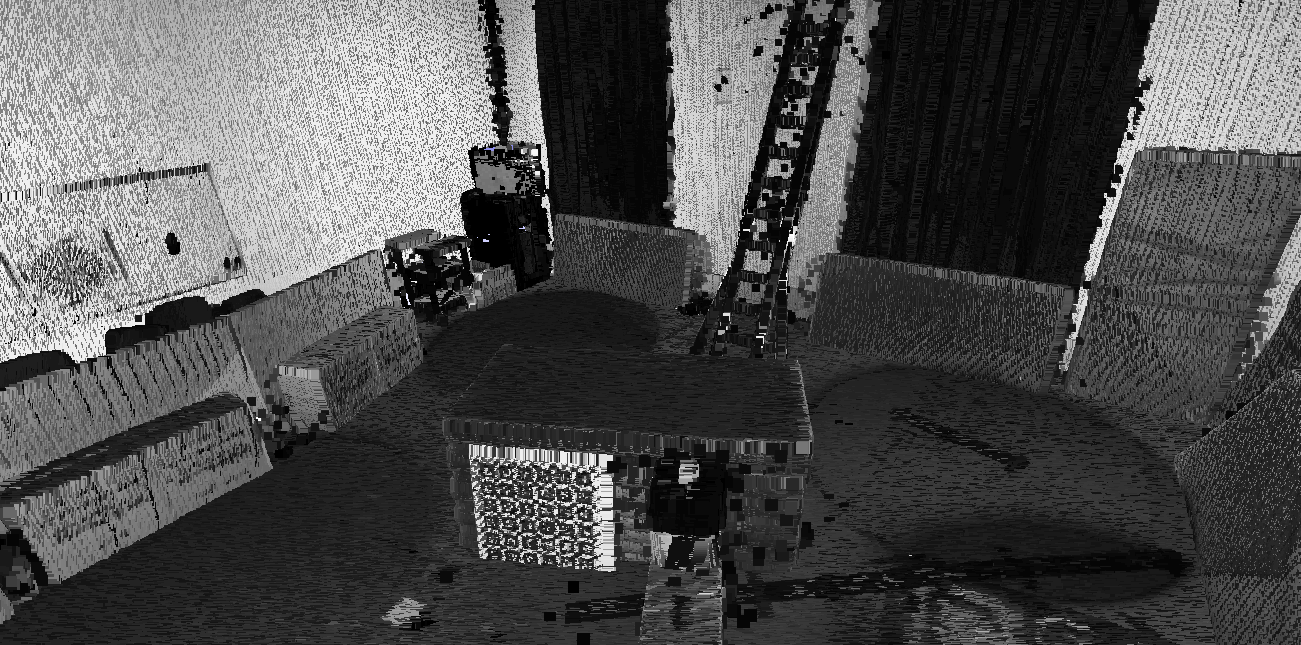
\includegraphics[scale=0.2]{Euroc/Pointcloud1.png}
	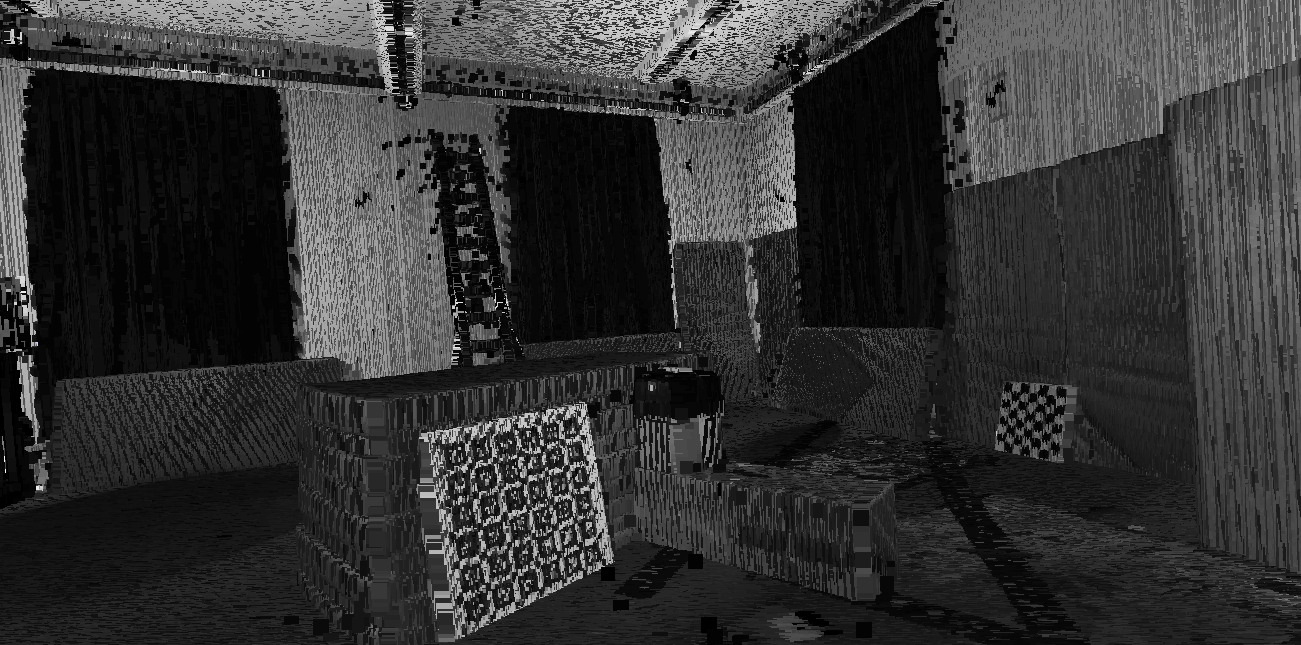
\includegraphics[scale=0.2]{Euroc/Pointcloud2.png}
	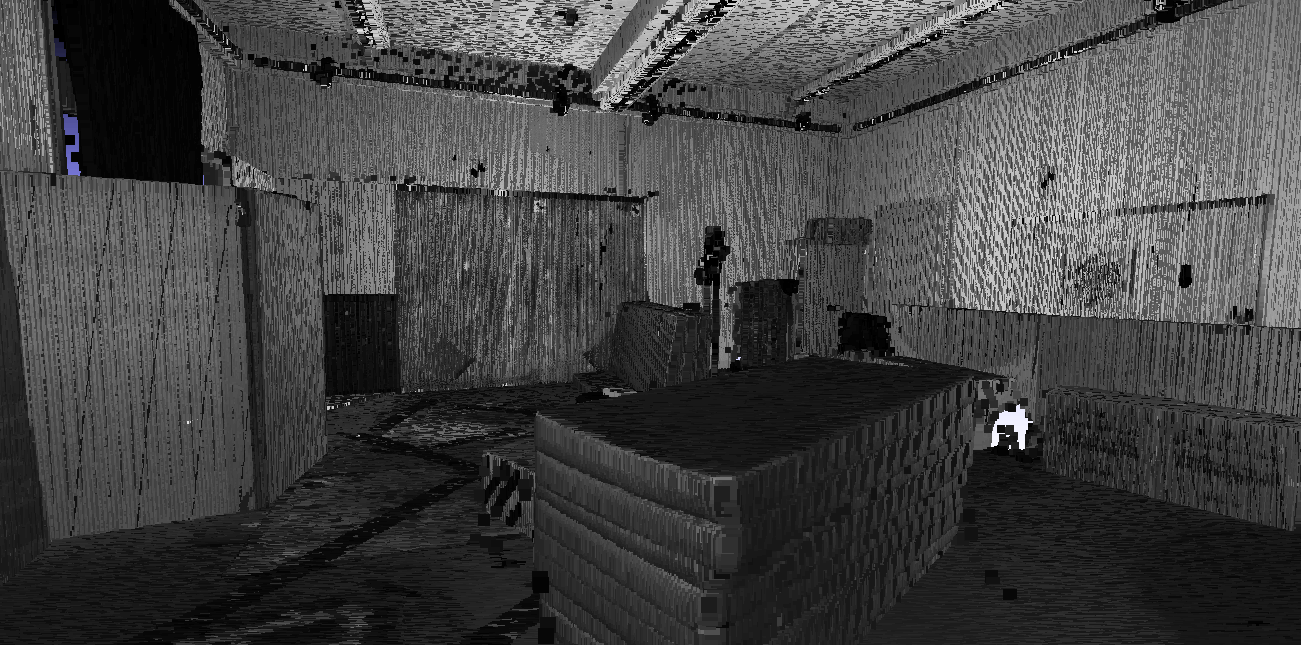
\includegraphics[scale=0.2]{Euroc/Pointcloud3.png}
	\caption[Nubes de puntos de la habitación utilizada en el EuRoC MAV Dataset]{Nubes de puntos de la habitación utilizada en el EuRoC MAV Dataset.}
	\label{fig:pointcloudEuroc}
\end{figure}

Cabe destacar que este dataset fue utilizado como referencia para la generación del dataset local del capítulo 5, conservando las mismas convenciones de formato.

\section{Tipología de implementación}

En el presente trabajo se propone un sistema de SLAM basado en la fusión visual-inercial,  capaz de integrar  la estimación de movimiento  proveniente de los métodos visuales semi-directos basados en cámara monocular, y la estimación de movimiento que se puede obtener de una unidad de medición inercial. La figura \ref{fig:esquemaGeneral} presenta el esquema básico propuesto.

\begin{figure}[H]
	\centering
	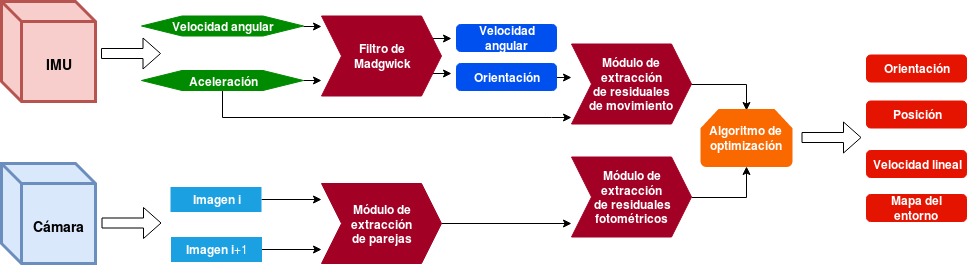
\includegraphics[scale=0.4]{Implementacion/DiagramaSistema.png}
	\caption[Esquema general del sistema implementado]{Esquema general del sistema implementado}
	\label{fig:esquemaGeneral}
\end{figure}

Este diagrama se encuentra dividido en los módulos del sistema inercial y los módulos del sistema visual, más el algoritmo de optimización fusiona  los datos provistos por estos módulos. Éste último tiene una vertiente basada en métodos directos, implementada previamente por \textit{Morales F.} \cite{fabio}, y una nueva versión, basada en un método de estimación con RANSAC.

En el caso del esquema inercial, se tiene un primer filtro de fusión de los datos de la IMU, el cual corresponde al filtro de Madgwick. Este filtro estima la orientación del sistema de la IMU respecto a un sistema fijo, partiendo de la velocidad angular y la aceleración medida. Posteriormente, se utiliza esta orientación para calcular los residuales inerciales. El sistema implementado también deja a disposición la posibilidad de utilizar otro filtro de fusión inercial como el filtro complementario.

En el esquema visual, el módulo de extracción de parejas se encarga de aplicar la detección de características en las imágenes de entrada y su emparejamiento. Estas parejas  son utilizadas para la extracción de los residuales fotométricos.

Finalmente, calculados los residuales inerciales y visuales,  el algoritmo de optimización estima la orientación, posición, velocidad, y un mapa del entorno a través de la triangulación en el espacio de las parejas detectadas.

La estimación de movimiento por medio de la fusión visual inercial fue desarrollada utilizando C++ como lenguaje de programación y ROS para la aplicación de los filtros inerciales y la visualización del movimiento del robot. Este programa utiliza un sólo hilo de ejecución, de forma que la odometría se estima de forma secuencial, pasando primero por estimar la orientación del robot utilizando el filtro inercial, y luego a estimar la traslación a partir de los residuales inerciales y la cámara. El formato de entrada de las imágenes y de los datos de la IMU fueron tomados de acuerdo al formato empleado en el EuRoC MAV dataset.



\section{Librería de desarrollo}

\subsection{OpenCV}

\begin{wrapfigure}{R}{5cm}
	\begin{center}
		\vspace*{-0.2in}
		
\includegraphics[width=4cm]{opencv}
	\end{center}
	\caption{Logo de la librería OpenCV}
\end{wrapfigure}

Para la implementación de los módulos previamente descritos, es necesario el uso de librerías y entornos de trabajo, que permitan un manejo eficiente de las imágenes. Además, el uso de de plataformas que se encuentren estandarizadas en esta área de estudio, facilita que el desarrollo del presente trabajo siga avanzando de la mano de futuros desarrolladores. En base a esto, se seleccionó la librería OpenCV\footnote{\url{http://opencv.org/}} para la implementación de los módulos necesarios en el sistema de generación de mosaico.

OpenCV (del inglés: \textit{Open Source Computer Vision}) es una librería de procesamiento de imágenes desarrollada por la empresa Intel\footnote{\url{http://www.intel.com}} en el año 1999. Esta librería ofrece un gran numero de algoritmos optimizados (actualmente mas de 2.500), el cual proporciona un entorno de desarrollo altamente eficiente para aplicaciones de procesamiento de imágenes. Asimismo presenta una gran aceptación por parte de los usuarios en el mundo académico y comercial, con mas de 47 mil usuarios activos, y un numero de descargas que supera los 14 millones. Se considera el estándar de facto en la comunidad de desarrolladores, y en especial para proyectos de investigación en procesamiento de imágenes y visión por computadora. 

Esta plataforma tiene soporte para distintos sistemas operativos, como \textit{Windows, Linux, Mac OS, iOS y Android.} Además de tener la posibilidad de trabajarla con diversos lenguajes de programación como: C++, Python, JavaScript. La motivación del presente trabajo se encuentra orientada al desarrollo de una aplicación que en un futuro pueda ser embebida en un sistema de navegación automático, con lo cual el soporte de un lenguaje de bajo nivel como C++, puede permitir el desarrollo de un algoritmo con suficiente velocidad de cómputo para este fin.

Por otra parte, esta librería presenta soporte para trabajar con la arquitectura de cálculo paralelo \textit{CUDA} (del inglés: \textit{Compute Unified Device Architecture}) de la empresa NVIDIA\footnote{\url{http://www.nvidia.com}}, con la cual se puede aprovechar el uso de las unidades de procesamiento gráfico para acelerar el rendimiento del algoritmo que se implemente. Cabe destacar que los equipos presentes en el laboratorio del \textit{GIDM} tienen disponible tarjetas gráficas con este soporte.

